\documentclass[11pt,a4paper]{article}

% -------------------------------------------------------
% PACKAGES
% -------------------------------------------------------
\usepackage{amsmath,amssymb,siunitx,graphicx,booktabs}
\usepackage{geometry}
\usepackage{caption}
\usepackage{datetime}
\usepackage{tabularx}
\usepackage{multirow}
\usepackage{float}
\usepackage{xcolor}
\usepackage{microtype} % nice typography
\usepackage{tikz}
\usetikzlibrary{arrows.meta, positioning}


\geometry{margin=1in}
\sisetup{detect-all}
\setlength{\parskip}{0.6em}
\setlength{\parindent}{0pt}

% Keep hyperref last
\usepackage{hyperref}
\hypersetup{
  colorlinks=true,
  linkcolor=blue!50!black,
  citecolor=blue!50!black,
  urlcolor=blue!60!black,
  pdfauthor={Salah-Eddin Gherbi},
  pdftitle={Photometric and Non-Gravitational Anomalies in 3I/ATLAS (C/2025 N1)}
}

\usepackage{fancyhdr}
\pagestyle{fancy}
\fancyfoot[L]{\scriptsize \href{https://doi.org/10.5281/zenodo.17692904}{DOI: 10.5281/zenodo.17692904}}
\fancyfoot[C]{\small \thepage}  % ← Slightly smaller page numbers
\fancyfoot[R]{\scriptsize © Salah-Eddin Gherbi (2025) — CC BY-NC 4.0}

% Also reset the header since \maketitle changes page style
\fancyhead{} % clear all header fields
\renewcommand{\headrulewidth}{0pt} % remove header line

% -------------------------------------------------------
% METADATA
% -------------------------------------------------------
\title{\textbf{Photometric and Non-Gravitational Anomalies in the Interstellar Object 3I/ATLAS (C/2025 N1)}}
\author{
  Salah-Eddin Gherbi\\
  \small Independent Researcher, United Kingdom\\
  \small ORCID: \href{https://orcid.org/0009-0005-4017-1095}{0009-0005-4017-1095}\\
  \small GitHub: \href{https://github.com/salahealer9/salah-gherbi-3I_ATLAS_Anomaly_2025}{salah-gherbi-3I\_ATLAS\_Anomaly\_2025}\footnote{The GitHub repository name contains the historical identifier ``C/2019~Y4'', which reflects an early internal naming convention used during the development of the analysis pipeline. This naming does \emph{not} refer to the comet C/2019~Y4 (ATLAS), and all datasets, scripts, and results in this study correspond exclusively to the interstellar object 3I/ATLAS (C/2025~N1).}
}
\date{\today}

% -------------------------------------------------------
\begin{document}
\maketitle
\thispagestyle{fancy}
\begin{abstract}
We report a photometric and chromatic analysis of the interstellar object \textbf{3I/ATLAS (C/2025 N1)} based on 4,580 Minor Planet Center observations spanning 2025-05-08 to 2025-11-21. Using a simple optical activity proxy derived from the time derivative of the inverse magnitude, we identify a pre-perihelion acceleration peak in early October 2025 (around 2025-10-02), roughly one month before perihelion. This enhanced optical activity is temporally coincident with a pronounced reddening of the $g-o$ colour index ($\Delta(g-o)\approx+0.7$~mag) during July–September, suggesting a coupled evolution of brightness and dust-dominated scattering. Post-perihelion photometry shows a reversal of the optical activity proxy and a transition into a fading phase, although multi-filter coverage is insufficient to track the corresponding colour evolution. Taken together, these results demonstrate that purely photometric monitoring can reveal pre-perihelion activity and post-perihelion relaxation in interstellar objects, and provide an independent temporal diagnostic complementary to dynamical non-gravitational terms. All data, analysis code, and verification artefacts are cryptographically timestamped and publicly archived.
\end{abstract}


\vspace{1em}

\textbf{Keywords:} 3I/ATLAS, interstellar objects, cometary photometry, non-gravitational acceleration, colour indices, outgassing dynamics

% =======================================================
\section{Introduction}
% =======================================================
The object \textbf{C/2025 N1 (ATLAS)}, recently designated as \textbf{3I/ATLAS}, is the third confirmed interstellar visitor to the Solar System.  
Initial astrometric solutions indicated a hyperbolic eccentricity of $e = 6.137 \pm 0.0006$ and an inclination of $i = 175.11^\circ$, suggesting an inbound trajectory nearly antiparallel to the ecliptic.  
Preliminary reports from JPL (Davide Farnocchia, 2025-10-29) introduced a small but significant non-gravitational term ($A_1 \approx 1.66\times10^{-6}\ \mathrm{au\,d^{-2}}$), implying active outgassing forces near perihelion.

This study investigates whether the reported non-gravitational acceleration is preceded or accompanied by measurable optical and chromatic anomalies.  
Photometric data from the Minor Planet Center (MPC) were analysed using a fully automated Python pipeline, producing daily averaged brightness, colour indices, and derived acceleration proxies.

% =======================================================
\section{Data and Methods}
% =======================================================
\subsection{Data Acquisition and Verification (v2.5)}
Raw MPC photometry for 3I/ATLAS was retrieved from:
\begin{verbatim}
https://www.minorplanetcenter.net/tmp2/3I.txt
\end{verbatim}
containing 4,580 lines spanning 2025-05-08 to 2025-11-21. 
The core photometric dataset and initial analysis pipeline are archived as \href{https://doi.org/10.5281/zenodo.17477597}{v2.5}~\cite{zenodoV25}.
All scripts and results were timestamped using \textbf{OpenTimestamps} and signed via GPG for reproducibility.  
A cryptographic run log (\texttt{RUN\_LOG.md}) maintains file hashes, statistical summaries, and blockchain proofs.

\subsection{Colour Indices}
Colour indices were computed from near-simultaneous multi-filter observations using MPC photometric bands (g, r, o, v, c).  
The principal diagnostic pairs were:
\[
(g - o), \quad (g - r), \quad (r - o)
\]
For each pair, rolling means and solar comparisons were derived:
\[
\Delta (X-Y) = \langle X-Y \rangle_{\text{ATLAS}} - (X-Y)_{\odot}
\]
with $(g-o)_\odot = 0.620$, $(g-r)_\odot = 0.440$, and $(r-o)_\odot = 0.180$.

\subsection{Optical Acceleration Proxy}
We define an optical activity proxy from the normalized flux derivative:
\[
A_\mathrm{opt}(t) = \frac{d}{dt}\left( \frac{1}{m(t)} \right) \approx \frac{\Delta (1/m)}{\Delta t}
\]
where $m(t)$ is the nightly mean magnitude. This quantity tracks changes in the brightening rate, serving as a photometric analog of physical acceleration when correlated with color changes.

\emph{Note:} $A_{\mathrm{opt}}$ is a photometric activity proxy derived from the temporal derivative of inverse magnitude. It is not a direct dynamical acceleration, but it correlates with phases of enhanced intrinsic brightening and thus complements orbital non–gravitational terms.

\subsection{Cross-Validation and External Data Check (v2.1)}

Version~2.1 of this analysis pipeline \href{https://doi.org/10.5281/zenodo.17483027}{(v2.1)}~\cite{zenodoV21} incorporated a cross-validation attempt using the
\textbf{Zwicky Transient Facility (ZTF) DR19} photometric archive via the IRSA TAP service.
No detections of 3I/ATLAS were reported between July and October~2025,
confirming that the anomaly remains uniquely recorded in MPC photometric data.

A fallback diagnostic plot (\texttt{I3\_MPC\_Only.png}) was generated to verify
that all brightness and colour trends originate solely from MPC sources.
The complete verification manifest (v2.1)---including the ZTF query logs, MPC dataset hash, and OpenTimestamps proofs---is archived on the Bitcoin blockchain and publicly available in the project's GitHub repository.

We summarize here the pre–perihelion brightening and reddening, and the first post–perihelion deceleration inferred from MPC photometry.

% =======================================================
\section{Results}
% =======================================================
\subsection{Solar Colour Comparison (July 2025)}
The early-phase colour indices (July) yielded:
\begin{align*}
(g-o) &= 0.723 \pm 0.463, & \Delta = +0.103 \,(\text{redder})\\
(g-r) &= 0.439 \pm 0.246, & \Delta = -0.001 \,(\text{solar-like})\\
(r-o) &= 0.115 \pm 0.135, & \Delta = -0.065 \,(\text{bluer})
\end{align*}
indicating a slightly red-shifted spectrum relative to solar but dominated by reflective scattering — consistent with icy surface composition.

\subsection{Optical Brightness and Acceleration}
The brightness evolution from May–November 2025 showed a monotonic increase in $1/m$ up to early October, where the optical acceleration proxy reached a sharp pre-perihelion maximum (Fig.~\ref{fig:accel}). The peak occurred around 2025-10-02, roughly one month before perihelion, with a scaled amplitude of order $10^{-3}$ in our proxy units.  
This timing is consistent with the onset of the non-gravitational term $A_1$ subsequently detected in orbital fits.

\begin{figure}[htbp]
  \centering
  \includegraphics[width=\textwidth]{I3_Optical_Acceleration_Trend_v2.png}
  \caption{\textbf{Optical vs Non-Gravitational Acceleration.}  
  The optical brightness (blue) rises smoothly until a pronounced change in the acceleration (red) around late September–early October 2025, preceding perihelion (dashed magenta).  
  This optical signature correlates temporally with the first reported non-gravitational term ($A_1 \approx 1.66\times10^{-6}$~au~d$^{-2}$).}
  \label{fig:accel}
\end{figure}


\subsection{Photometric Anomaly and Flux Increase (v2.0)}

Between July and October 2025, 3I/ATLAS displayed a smooth, monotonic increase in mean brightness from
$V \approx 17.3 \pm 1.0$~mag to $V \approx 13.1 \pm 0.6$~mag,
corresponding to a total brightening of $\Delta m \approx 4.2$~mag—
a flux increase of roughly $\times 47$.
This change occurred over only $\sim90$~days and is far greater than can be accounted for by geometric effects
(heliocentric or geocentric distance, or phase‐angle variation), which would predict at most $\sim1.5$~mag.

The amplitude and continuity of the brightening therefore constitute a photometric anomaly: a departure from purely reflective or geometric behaviour,implying an intrinsic increase in the object's optical output.
Possible explanations include renewed outgassing or volatile release as the body re‐emerged from solar conjunction,
the exposure of fresh icy material through fragmentation or rotational resurfacing, or a combination of both.

The dataset used here is derived directly from Minor Planet Center observational records (\texttt{I3.txt})
and processed without interpolation or external photometric calibration,ensuring that the observed trend reflects the raw reported magnitudes.
The Horizons comparison extension is archived as \href{https://doi.org/10.5281/zenodo.17483027}{v2.0}~\cite{zenodoV2}.
Because all files are timestamp‐verified via \textbf{OpenTimestamps}, the results are independently auditable and temporally authenticated.

Future comparison with forthcoming astrometric and spectroscopic datasets will clarify whether this brightening represents a transient outburst phase
or a longer‐term reactivation of residual ices.
Either interpretation identifies 3I/ATLAS as a dynamically evolving body exhibiting post‐conjunction activity inconsistent with a purely inert interstellar nucleus.

\enlargethispage{\baselineskip}
\subsection{Chromatic Evolution and Reddening Transition}
The temporal coincidence of optical acceleration with color evolution (Fig.~\ref{fig:colorcorr}) shows a reddening of $\Delta(g-o) = +0.57$~mag during the acceleration window. This chromatic shift \textbf{suggests} a transition from reflective icy scattering to dust emission, though the specific mechanism requires further investigation.

\begin{figure}[htbp]
  \centering
  \includegraphics[width=\textwidth]{I3_Optical_Color_Correlation.png}
\caption{\textbf{Pre-Perihelion Optical Acceleration and Colour Evolution.}  
Left: optical brightness (blue) and scaled acceleration (red) showing a pre-perihelion surge.  
Right: $g-o$ colour index evolution (July 1–September 11) showing early bluing followed by reddening ($\Delta = +0.57$~mag) during the acceleration window (cyan).  
\textit{Note: Color data coverage ends September 11; photometry continues through November 21.}}
  \label{fig:colorcorr}
\end{figure}

Color indices are available through 2025-09-11; subsequent photometry to 2025-11-21 lacks simultaneous multi-filter coverage.

% =======================================================
\subsection{Spectral Transition and Colour Evolution}
% =======================================================
The colour index \( (g-o) \) measures the relative brightness between green and orange filters:
\[
(g-o) = m_g - m_o,
\]
where larger values indicate a fainter green component (redder spectrum), while smaller values indicate enhanced green emission (bluer spectrum).  
For reference, the solar colour baseline is \( (g-o)_\odot \approx 0.62 \).

Table~\ref{tab:color_evolution} summarizes the mean monthly evolution of 3I/ATLAS during its approach to perihelion:

\begin{table}[H]
\caption{Evolution of the \( g-o \) Colour Index (vs Solar Baseline \( 0.62 \))}
\begin{tabularx}{1.0\linewidth}{lccc}
\toprule
\textbf{Month (2025)} & \textbf{Mean \( g-o \)} & \textbf{\(\Delta (g-o)\)} & \textbf{Interpretation} \\
\midrule
July & 0.61 & $\approx 0$ & Neutral / reflective surface (icy scattering) \\
August & 0.94 & +0.32 & Reddening onset — dust or organic activation \\
September & 1.34 & +0.72 & Strong reddening — peak outgassing activity \\
October–November & \textit{No data} & \textit{No data} & \textit{Multi-filter coverage ended Sept 11} \\
\bottomrule
\end{tabularx}
\label{tab:color_evolution}
\end{table}

The progressive reddening from July to September coincides with the rise toward the revised pre-perihelion optical acceleration peak, which the extended MPC dataset places on 2025-10-02. This indicates that photometric brightening and chromatic alteration arise from the same physical process: the release of large, carbonaceous dust grains and complex organic material. Such reddening reflects enhanced absorption at shorter wavelengths, consistent with tholin-like or hydrocarbon mantling as the nucleus surface was irradiated by sunlight and solar wind.

After perihelion (late October–early November), the optical acceleration reversed (\( \mathrm{A_{opt}} < 0 \)), suggesting the fading of outgassing and the dispersal of the dense dust coma.  
A corresponding return toward bluer colours is therefore expected as the transparent gas halo and solar scattering begin to dominate once more.

This neutral → red → fading transition forms a distinct spectral fingerprint of the object’s activity cycle and may indicate a non-terrestrial dust composition, darker and more carbonized than typical solar-system comets.

The post-perihelion evolution is illustrated in Figure~\ref{fig:postperi}, which shows the monotonic fading and sustained negative optical acceleration following the 2025-10-29 perihelion passage.

\begin{figure}[htbp]
  \centering
  \includegraphics[width=\textwidth]{I3_Optical_Color_Correlation_postperi.png}
  \caption{\textbf{Post-Perihelion Optical Evolution (2025-10-29 to 2025-11-21).}  
  Optical brightness (blue) and acceleration proxy (red) showing the transition to fading phase post-perihelion (dashed magenta line).  
  The acceleration reversal (\(A_{\mathrm{opt}} < 0\)) indicates decreasing brightening rate as the object moves away from the Sun. Photometric coverage extends to 2025-11-21, capturing the post-perihelion fading phase with improved temporal resolution. \textit{Note: Color indices unavailable post-perihelion due to limited multi-filter coverage; plot shows photometric evolution only.} The extended photometric coverage through 2025-11-21 confirms a strictly monotonic fading with a stable negative optical acceleration, and shows no evidence for secondary activation or additional dynamical anomalies.
}
  \label{fig:postperi}
\end{figure}

\subsection{Data Coverage and Limitations}
Photometric observations span 2025-05-08 to 2025-11-21 with 120 unique observing nights. A multi-week observational gap occurred in mid–October due to the object's close solar approach, which is typical for inner Solar System targets. Color analysis was performed on simultaneous multi-filter observations from 2025-07-01 to 2025-09-11 (67 measurements). The acceleration analysis utilizes all available photometry, with natural observational gaps preserved to maintain data integrity.

\subsection{Post-Perihelion Update (November 2025)} 

Extended MPC photometry through 2025-11-21 provides the first glimpse of post-perihelion behaviour. The optical acceleration proxy changes sign from positive values near the pre-perihelion peak to negative values in early November, marking a transition from intensifying activity to gradual optical fading as the object recedes from solar proximity.

\paragraph{Extended post-perihelion evolution (2025-11-13 to 2025-11-21).}
The inclusion of the most recent MPC photometry (extending the dataset to 2025-11-21) reveals that 3I/ATLAS continues to fade smoothly after perihelion. The inverse-magnitude brightness $1/m$ declines approximately linearly, with no evidence of secondary brightening or renewed activity. The optical acceleration proxy remains consistently negative, fluctuating in the range $\sim(-2$--$-3)\times 10^{-3}$ in scaled units, indicating that the object has entered a quasi-inert regime. This behaviour supports the interpretation that the activation episode was brief and did not evolve into sustained outgassing. The absence of curvature, plateaus, or additional acceleration pulses strengthens the conclusion that the post-perihelion evolution is governed by passive dust dispersal rather than active mass loss.

\textbf{Spectral coverage limitations:} While photometric data extend to 2025-11-21, the multi-filter observations required for colour indices ceased after 2025-09-11. This prevents direct confirmation of post-perihelion chromatic evolution, though the pre-perihelion data already demonstrate a robust correlation between reddening and optical acceleration. 

The observed deceleration phase is consistent with a fading of surface activity or with geometric and phase-angle effects following perihelion passage. However, the timing and amplitude of the preceding reddening event (\(\Delta(g-o)\!\approx\!+0.7~\mathrm{mag}\)) remain atypically large for a solar-system-like body. The most neutral interpretation is that 3I/ATLAS underwent a transient release or reconfiguration of surface material whose optical properties evolved with solar irradiation. 

Whether this behaviour represents volatile loss, dust scattering changes, or other mechanisms intrinsic to an interstellar nucleus cannot yet be established. Continued photometric monitoring will clarify whether the object stabilizes or undergoes further variations as it exits the inner Solar System.

% =======================================================
\section{Discussion}
The correlated reddening and acceleration \textbf{appear consistent with} natural outgassing processes, where larger dust grains could produce both the observed color change and non-gravitational forces. However, several aspects merit caution:

\begin{itemize}
\item The \textbf{sharp temporal definition} of the acceleration window (around 2025-10-02$\pm$3 days) shows unusual precision for stochastic natural outbursts
\item The \textbf{reddening signature} differs from typical cometary bluing during ice sublimation
\item The \textbf{amplitude of color change} ($\Delta = +0.57$ mag) is substantial for a single event
\end{itemize}

While natural explanations remain most probable given Occam's Razor, the anomalous characteristics justify keeping alternative interpretations in consideration until more interstellar objects are observed with similar instrumentation.

\subsection{Independent Observational Confirmation}
Recent independent imaging from the R. Naves Observatory (2025-11-05) confirms the post-perihelion behavior identified in this analysis. The observation shows 3I/ATLAS as a "fuzzy ball of light" without obvious cometary tail structure \cite{naves2025}, consistent with our finding of optical fading and acceleration reversal. This independent validation supports the interpretation of declining dust production and the absence of sustained cometary activity post-perihelion.

In addition, new post-perihelion images obtained with the 2.6-m Nordic Optical Telescope (NOT) on 2025-11-09 independently corroborate this behaviour (Fig.~\ref{fig:not_observations}). The NOT frames show a compact, unresolved central condensation with no evidence of fragmentation and no detectable dust tail or asymmetric coma structure. The morphology is point-like at all wavelengths and signal-to-noise levels, consistent with a weakly active or inactive body.

This independently confirms the post-perihelion optical fading and acceleration reversal identified in this analysis (Figs.~\ref{fig:accel}, \ref{fig:postperi}). Unlike ordinary comets—which typically exhibit a prominent dust coma or tail after perihelion—3I/ATLAS appears morphologically stellar. This supports the interpretation that the strong pre-perihelion reddening event was transient and did not lead to sustained cometary outgassing.

\subsection{Nature Classification Uncertainty}
The fundamental nature of 3I/ATLAS remains ambiguous. While our analysis reveals photometric and chromatic behavior consistent with transient cometary activity—specifically dust-driven reddening and subsequent fading—the object lacks clear spectroscopic or morphological signatures of typical cometary outgassing. Recent imaging showing no detectable tail \cite{naves2025} further complicates classification.

\clearpage

\begin{figure}[htbp]
\centering

% First row
\begin{minipage}{0.4\textwidth}
    \centering
    \includegraphics[width=\linewidth,page=1]{NOTpictures.pdf}
    \vspace{0.1cm}
    \textbf{(a) Linear stretch}
\end{minipage}
\hfill
\begin{minipage}{0.4\textwidth}
    \centering
    \includegraphics[width=\linewidth,page=2]{NOTpictures.pdf}
    \vspace{0.1cm}
    \textbf{(b) Contoured}
\end{minipage}

\vspace{0.3cm}

% Second row  
\begin{minipage}{0.4\textwidth}
    \centering
    \includegraphics[width=\linewidth,page=3]{NOTpictures.pdf}
    \vspace{0.1cm}
    \textbf{(c) Color contoured}
\end{minipage}
\hfill
\begin{minipage}{0.4\textwidth}
    \centering
    \includegraphics[width=\linewidth,page=4]{NOTpictures.pdf}
    \vspace{0.1cm}
    \textbf{(d) Spatially filtered}
\end{minipage}

\caption{
\textbf{Multi-analysis of 3I/ATLAS from NOT on 2025-11-11} --- 
\textbf{(a) Linear:} Sunward-pointing jet in raw image; 
\textbf{(b) Contoured:} Enhanced morphological detail; 
\textbf{(c) Color:} Spectral overlay; 
\textbf{(d) Filtered:} Median-subtracted within 0.13 million km radius. 
North up, East left; field spans 0.5 million km. Marked: anti-solar ($-S$) and velocity ($-V$) directions. Upper-left diffuse object is a background galaxy; other sources are stars. These NOT observations show sunward activity without extended cometary features, consistent with transient acceleration events identified here. \textbf{Source:} \cite{atel17490}.
}
\label{fig:not_observations}
\end{figure}

This ambiguity highlights the challenge of characterizing interstellar objects with limited observational data. 3I/ATLAS may represent:
\begin{itemize}
\item A \textbf{weakly active comet} with minimal gas production
\item A \textbf{dust-dominated body} experiencing surface modification
\item A \textbf{transitional object} between asteroid and comet classifications
\item An \textbf{exotic composition} unlike solar system analogues
\end{itemize}

The absence of definitive cometary features, coupled with clear photometric anomalies, suggests 3I/ATLAS may belong to a previously unobserved class of interstellar objects where traditional Solar System taxonomy proves inadequate.

Furthermore, the NOT images strongly constrain any model requiring sustained outgassing or nucleus disruption. At a phase where cometary nuclei normally display extended dust comae, 3I/ATLAS remains unresolved and tail-less. This observational constraint, combined with the photometric deceleration, suggests that any activity was short-lived and that the object presently behaves as a largely inert interstellar body.

\subsection{Context of Multiple Independent Anomalies}

The photometric–chromatic anomalies identified in this work must be considered within the broader context of \textit{3I/ATLAS}'s unprecedented characteristics documented by Loeb \emph{et~al.}~\cite{loeb2025atlas}. These independent anomalies include several distinct classes:

\subsubsection{Orbital and Dynamical Anomalies}

\begin{itemize}
  \item \textbf{Precise orbital alignment:} Retrograde trajectory aligned within \(5^{\circ}\) of the ecliptic plane (probability \(\approx 0.2\%\)).
  \item \textbf{Arrival timing fine-tuning:} Trajectory optimized for close planetary encounters (Mars, Venus, Jupiter) while avoiding direct Earth observation at perihelion (probability \(\approx 0.005\%\)).
  \item \textbf{Non-gravitational acceleration:} Significant acceleration detected at \(3.7\sigma\) confidence, with radial and transverse components of \(1.1\times10^{-6}\,\mathrm{au\,day^{-2}}\) and \(3.7\times10^{-7}\,\mathrm{au\,day^{-2}}\), respectively.
  \item \textbf{Mass-loss requirement:} The inferred non-gravitational acceleration implies \(>13\%\) mass loss during perihelion passage if driven solely by natural cometary outgassing.
\end{itemize}

\subsubsection{Physical and Compositional Anomalies}

\begin{itemize}
  \item \textbf{Extreme mass and velocity:} Nucleus estimated to be \(\sim10^{6}\!\times\) more massive than 1I/\textquoteleft Oumuamua and \(\sim10^{3}\!\times\) more massive than 2I/Borisov, while exhibiting higher inbound velocity (probability \(<0.1\%\)).
  \item \textbf{Unusual composition:} Gas plume contains nickel-rich material with \(\mathrm{Ni:Fe}\) ratios resembling industrial alloys and \(\mathrm{Ni:CN}\) ratios several orders of magnitude higher than known cometary values (probability \(<1\%\)).
  \item \textbf{Anomalous jet structure:} A sunward anti-tail observed between July and August~2025 is inconsistent with geometric perspective effects in ordinary comets.
\end{itemize}

\subsubsection{Photometric and Evolutionary Anomalies}

\begin{itemize}
  \item \textbf{Extreme perihelion brightening:} Brightness increased by a factor of \(\sim5\) in the green band (\(0.464~\mu\mathrm{m}\)) near perihelion.
  \item \textbf{Bluish coloration:} An unusually blue spectral slope near perihelion, inconsistent with typical cometary reddening.
  \item \textbf{Timing of acceleration onset:} Detectable non-gravitational acceleration appeared only after September~2025, despite \(4{,}022\) pre-perihelion observations showing no such effect.
\end{itemize}

\begin{table}[H]
\centering
\scriptsize
\setlength{\tabcolsep}{3pt}
\caption{Summary of Independent Anomalies Observed in \textit{3I/ATLAS} (C/2025~N1)}
\begin{tabularx}{\linewidth}{lXcc}
\toprule
\textbf{Category} & \textbf{Observation / Description} & \textbf{Estimated Probability} & \textbf{Reference} \\
\midrule
\textbf{Orbital–Dynamical} 
  & Retrograde orbit aligned within \(5^{\circ}\) of the ecliptic plane & \(\sim0.2\%\) & \cite{loeb2025atlas} \\
  & Arrival timed for near-encounters (Mars, Venus, Jupiter) while avoiding Earth at perihelion & \(\sim0.005\%\) & \cite{loeb2025atlas} \\
  & Non-gravitational acceleration (\(1.1\times10^{-6}\)~radial, \(3.7\times10^{-7}\)~transverse~\(\mathrm{au\,day^{-2}}\)) at \(3.7\sigma\) significance & — & \cite{loeb2025atlas} \\
  & Required mass loss \(>13\%\) if due to outgassing & — & \cite{loeb2025atlas} \\

\textbf{Physical–Compositional} 
  & Nucleus mass \(\sim10^{6}\!\times\) 1I/\textquoteleft Oumuamua, \(\sim10^{3}\!\times\) 2I/Borisov; higher inbound velocity & \(<0.1\%\) & \cite{loeb2025atlas} \\
  & Nickel-rich gas plume (\(\mathrm{Ni:Fe}\) $\approx$ industrial alloys; \(\mathrm{Ni:CN}\) ratios orders of magnitude above cometary norms) & \(<1\%\) & \cite{loeb2025atlas} \\
  & Sunward anti-tail observed (July–August~2025), inconsistent with geometric projection effects & — & \cite{loeb2025atlas} \\

\textbf{Photometric–Evolutionary} 
  & Perihelion brightening by factor \(\sim5\) in Green band (\(0.464~\mu\mathrm{m}\)) & — & \cite{loeb2025atlas} \\
  & Bluish coloration near perihelion (inverse of typical cometary reddening) & — & \cite{loeb2025atlas} \\
  & Onset of non-gravitational acceleration only post-September despite \(4{,}022\) pre-perihelion observations showing none & — & \cite{loeb2025atlas} \\
  & \textbf{Photometric correlation between optical acceleration proxy and \(g-o\) color reddening (new empirical finding)} & — & \textbf{This paper} \\

\textbf{Morphological}
  & Post-perihelion NOT images show point-like morphology (no coma or tail); inconsistent with sustained cometary outgassing & — & NOT (2025) \\
\bottomrule
\end{tabularx}

\vspace{2mm}
\raggedright
\footnotesize\textit{Note.}---Probabilities estimated from orbital simulation and compositional likelihood models. References denote original reporting of anomalies (Loeb \emph{et al.}, 2025); ``this paper'' indicates the newly reported photometric--chromatic correlation identified in the present analysis. The photometric correlation finding presented in this work independently confirms and extends the morphological anomaly reported by the Nordic Optical Telescope (NOT~2025), providing multi-wavelength evidence for atypical activity in 3I/ATLAS.
\label{tab:anomalies_summary}
\end{table}

The coordinated optical changes we detected add another photometric anomaly to this pattern of improbable traits. The combined likelihood of these anomalies challenges conventional astrophysics and warrants considering alternative explanations. Table~\ref{tab:anomalies_summary} summarizes the distinct anomalies reported to date for 3I/ATLAS, highlighting the newly identified optical–chromatic coupling presented in this work.

\subsection{Non--Gravitational \texorpdfstring{$\Delta v$}{Delta v} and the Jupiter Encounter Geometry} \label{sec:jupiter_dv}

To assess whether the optical–acceleration anomaly could influence the trajectory of 3I/ATLAS, we convert the dimensionless proxy $A_{\mathrm{opt}}(t)$ into an integrated non–gravitational impulse $\Delta v(t)$ using two physically motivated amplitude scalings:

\begin{enumerate}
    \item \textbf{Minimal case:} $\Delta v_{\mathrm{tot}} = 8~\mathrm{m\,s^{-1}}$, the amount required to reproduce the $\sim 10^{5}$~km displacement invoked in Loeb’s Jupiter–encounter geometry.
    \item \textbf{Photometric case:} $\Delta v_{\mathrm{tot}} = 25~\mathrm{m\,s^{-1}}$, consistent with the fitted $A_1$ parameter and the amplitude of the 
    two observed optical–acceleration peaks.
\end{enumerate}

In both cases, the \emph{shape} of $\Delta v(t)$ is determined entirely by the photometry; only the global amplitude differs. As Fig.~\ref{fig:dv_spikes} shows, nearly all the impulse originates from two brief activity spikes on 2025-09-10 and 2025-10-02, which together account for more than 90\% of the integrated momentum in both
normalisations.

\begin{figure}[htbp]
  \centering
  \includegraphics[width=\textwidth]{I3_Optical_Acceleration_DeltaV_Figure.png}
  \caption{\textbf{Time-resolved non–gravitational impulse.} 
  Two short-lived activity spikes dominate the total $\Delta v$ budget
  in both scaling regimes.}
  \label{fig:dv_spikes}
\end{figure}

The cumulative impulses for the two scalings are compared in
Fig.~\ref{fig:dv_overlay}. The curves share the same temporal structure, differing only by a scale factor. This indicates that the time-dependence of the impulse is robustly constrained by the optical data, regardless of interpretation.

\begin{figure}[htbp]
  \centering
  \includegraphics[width=\textwidth]{I3_Optical_Acceleration_DeltaV_Overlay.png}
  \caption{\textbf{Cumulative non–gravitational $\Delta v(t)$ for two normalisations.}  
  The minimal (8~m\,s$^{-1}$) and photometric (25~m\,s$^{-1}$) curves have identical timing and shape, differing only in amplitude.} 
  \label{fig:dv_overlay}
\end{figure}

Using $\Delta v_\perp = \Delta v_{\mathrm{tot}}\sin\theta$ at
$\theta = 30^\circ, 60^\circ, 90^\circ$ and propagating the resulting offset to Jupiter’s distance, the minimal case yields transverse displacements of $\sim(0.05$–$0.10)\times10^{6}~\mathrm{km}$, consistent with Loeb’s required $\sim 10^{5}$~km adjustment. The photometric case predicts proportionally larger offsets, $\sim(0.16$–$0.31)\times10^{6}$~km.

The resulting transverse components and propagated offsets are summarised in Table~\ref{tab:jupiter_dv_offsets}.

\begin{table}[htbp]
\centering
\caption{\textbf{Transverse non–gravitational impulse and resulting lateral displacement $\Delta b$ at Jupiter for two $\Delta v$ scalings.} The minimal ($8~\mathrm{m\,s^{-1}}$) case corresponds to the displacement required by Loeb’s Jupiter–encounter geometry, while the $25~\mathrm{m\,s^{-1}}$ case reflects the magnitude implied by the fitted non–gravitational parameter $A_1$.}
\label{tab:jupiter_dv_offsets}

\begin{tabular}{cccccc}
\toprule
\textbf{Case} & $\mathbf{\Delta v_{\mathrm{tot}}}$ (m/s) 
& $\mathbf{\theta}$ (deg) 
& $\mathbf{\Delta v_\perp}$ (m/s) 
& $\mathbf{\Delta b}$ (km) \\ 
\midrule

\multirow{3}{*}{Minimal} 
& \multirow{3}{*}{8.00}
& 30 & 4.00  & 49\,866 \\
& & 60 & 6.93 & 86\,370 \\
& & 90 & 8.00 & 99\,732 \\

\midrule

\multirow{3}{*}{Photometric}
& \multirow{3}{*}{25.00}
& 30 & 12.50 & 155\,831 \\
& & 60 & 21.65 & 269\,907 \\
& & 90 & 25.00 & 311\,662 \\

\bottomrule
\end{tabular}
\end{table}

These results show that the perihelion optical–acceleration anomaly has the dynamical capacity to induce a trajectory perturbation of the size associated with the proposed Jupiter geometry. Whether such an impulse arises from natural activity, an unusual physical mechanism, or a more complex process remains an open question.

% =======================================================
\subsection{Interstellar Anomaly Index for 3I/ATLAS}
\label{sec:anomaly_index}
% =======================================================

The preceding sections demonstrate that 3I/ATLAS exhibits anomalies in several independent observables: photometric brightening, colour evolution, non-gravitational acceleration, and post-perihelion morphology. In order to summarise these deviations in a single quantitative framework, we introduce an empirical \emph{Interstellar Anomaly Index} (IAI). This index is not intended to measure artificiality directly; rather, it compresses multi-dimensional deviation from typical cometary behaviour into a dimensionless score on the interval $[0,1]$, where $0$ corresponds to ordinary comets and $1$ to objects that are highly anomalous on several axes.

\subsubsection{Definition of the Index}

We consider four primary anomaly components:
\begin{enumerate}
    \item $A_{\mathrm{p}}$: \textbf{photometric anomaly}, based on excess brightening relative to geometric expectations;
    \item $A_{\mathrm{c}}$: \textbf{chromatic anomaly}, based on the amplitude of colour-index 
    variation relative to typical cometary evolution;
    \item $A_{\mathrm{a}}$: \textbf{acceleration anomaly}, incorporating the detection and timing of non-gravitational acceleration relative to photometric activity;
    \item $A_{\mathrm{m}}$: \textbf{morphological anomaly}, describing the discrepancy between the inferred activity level and the observed coma/tail morphology.
\end{enumerate}

Each component $A_i$ is normalised to lie in $[0,1]$, with $0$ indicating behaviour consistent with well-studied Solar System comets and $1$ indicating a strongly atypical value. 
The overall anomaly index is then defined as a weighted linear combination:
\begin{equation}
    \mathrm{IAI} = \sum_{i} w_i A_i,
\end{equation}
with $\sum_i w_i = 1$ and $w_i \geq 0$. In this initial implementation we adopt equal weights,
\begin{equation}
    w_{\mathrm{p}} = w_{\mathrm{c}} = w_{\mathrm{a}} = w_{\mathrm{m}} = \frac{1}{4},
\end{equation}
and discuss alternative weighting schemes in future work.

\subsubsection{Component Metrics}

The individual components are defined in terms of observable quantities as follows.

\paragraph{Photometric anomaly $A_{\mathrm{p}}$.}
Let $\Delta m_{\mathrm{obs}}$ denote the observed brightening between an early and late epoch (e.g., July--October 2025), and $\Delta m_{\mathrm{geo}}$ the brightening expected from heliocentric and geocentric distance variations and phase-angle effects alone. We define the photometric ratio
\begin{equation}
    R_{\mathrm{phot}} = \frac{\Delta m_{\mathrm{obs}}}{\Delta m_{\mathrm{geo}}},
\end{equation}
and map it to $[0,1]$ using a capped linear transformation:
\begin{equation}
    A_{\mathrm{p}} = \min\left(1,\; \frac{R_{\mathrm{phot}} - 1}{2}\right),
\end{equation}
so that purely geometric brightening ($R_{\mathrm{phot}} \approx 1$) yields $A_{\mathrm{p}}\approx 0$, while $R_{\mathrm{phot}} \gtrsim 3$ saturates at $A_{\mathrm{p}} \approx 1$. For 3I/ATLAS we measure $\Delta m_{\mathrm{obs}} \approx 4.2$\,mag and $\Delta m_{\mathrm{geo}} \approx 1.5$\,mag (Section~3.3), implying $R_{\mathrm{phot}} \approx 2.8$ and $A_{\mathrm{p}}\approx 0.9$.

\paragraph{Chromatic anomaly $A_{\mathrm{c}}$.}
Let $\Delta_{\mathrm{color}}$ denote the maximum excursion in the $g-o$ colour index relative to the solar baseline over the observational window ($\Delta_{\mathrm{color}} \approx 0.72$\,mag for 3I/ATLAS; Table~1). We adopt a reference range of $\sim 0.2$\,mag as typical for Solar System 
comets and define
\begin{equation}
    A_{\mathrm{c}} = \min\left(1,\; \frac{\Delta_{\mathrm{color}} - 0.2}{0.5}\right),
\end{equation}
such that modest colour evolution ($\Delta_{\mathrm{color}} \lesssim 0.2$) maps to $A_{\mathrm{c}}\approx 0$, while $\Delta_{\mathrm{color}} \gtrsim 0.7$ is considered strongly anomalous and saturates the scale. With $\Delta_{\mathrm{color}} \approx 0.72$\,mag, 3I/ATLAS attains $A_{\mathrm{c}} \approx 1$.

\paragraph{Acceleration anomaly $A_{\mathrm{a}}$.}
The acceleration anomaly combines (i) the detection of a non-gravitational term and 
(ii) the temporal offset between photometric and dynamical signatures. We introduce a binary indicator $B_{\mathrm{ng}}$ that is $1$ if a non-gravitational acceleration is detected at $>3\sigma$ significance and $0$ otherwise, and define
\begin{equation}
    T = \min\left(1,\; \frac{\Delta t}{30~\mathrm{days}}\right),
\end{equation}
where $\Delta t$ is the absolute time difference between the peak in the optical activity proxy (Section~3.2) and the epoch at which the non-gravitational term is first detected in orbital fits.
The acceleration anomaly is then
\begin{equation}
    A_{\mathrm{a}} = \frac{1}{2} B_{\mathrm{ng}} + \frac{1}{2} T.
\end{equation}
For 3I/ATLAS, $B_{\mathrm{ng}} = 1$ and $\Delta t \sim 30$\,days, giving $T \approx 1$ and 
$A_{\mathrm{a}} \approx 1$.

\paragraph{Morphological anomaly $A_{\mathrm{m}}$.}
Finally, we encode the discrepancy between the inferred activity level and the observed coma/tail 
structure in an ordinal parameter $\ell \in [0,1]$:
\begin{itemize}
    \item $\ell = 0$: classic cometary morphology with a well-developed coma and tail consistent 
   with the level of activity implied by photometry;
    \item $\ell = 0.5$: weak coma and marginal tail, partially consistent with the inferred activity;
    \item $\ell = 1$: point-like, asteroid-like morphology despite strong indications of recent 
    outgassing or mass loss.
\end{itemize}
The morphological anomaly is then 
\begin{equation}
    A_{\mathrm{m}} = \ell.
\end{equation}
Post-perihelion NOT images of 3I/ATLAS show a compact, stellar profile with no detectable tail 
or extended coma (Section~4.1), despite the implied pre-perihelion activity, motivating a value 
of $A_{\mathrm{m}} \approx 0.9$.

\subsubsection{Result for 3I/ATLAS}

Combining the above components with equal weights yields
\begin{equation}
    \mathrm{IAI}_{\mathrm{ATLAS}} = \frac{A_{\mathrm{p}} + A_{\mathrm{c}} + A_{\mathrm{a}} + A_{\mathrm{m}}}{4}
    \approx \frac{0.9 + 1.0 + 1.0 + 0.9}{4} \approx 0.95.
\end{equation}
On this heuristic scale, 3I/ATLAS lies close to the maximally anomalous end ($\mathrm{IAI}\approx 1$). 
We emphasise that this does \emph{not} constitute evidence of artificial origin. Instead, it quantifies the degree to which the object’s behaviour deviates from the envelope defined by well-characterised Solar System comets. In this sense, the Interstellar Anomaly Index complements the qualitative discussion of independent anomalies in Section~4.3 and provides a compact metric for comparing future interstellar objects observed with similar instrumentation.

\subsubsection{Position of 3I/ATLAS in the \texorpdfstring{$(e, \mathrm{IAI})$}{(e, IAI)} Plane}

To place 3I/ATLAS in a broader dynamical–anomaly context, we compare its Interstellar Anomaly Index with the orbital eccentricities of representative Solar System comets, 
along with the first two interstellar visitors 1I/'Oumuamua and 2I/Borisov. Figure~\ref{fig:iai_vs_e} shows that typical Jupiter-family and long-period comets cluster in the region $e \lesssim 1$ with $\mathrm{IAI} \lesssim 0.3$, while interstellar objects occupy $e > 1$. 3I/ATLAS lies in the extreme corner of this plane, with both very high eccentricity ($e \approx 6.14$) and a near-maximal anomaly index ($\mathrm{IAI} \approx 0.95$).

\begin{figure}[htbp]
    \centering
    \includegraphics[width=0.65\textwidth]{iai_vs_eccentricity.png}
    \caption{Interstellar Anomaly Index (IAI) as a function of orbital eccentricity for representative Solar System comets, 1I/'Oumuamua, 2I/Borisov, and 3I/ATLAS. The IAIs for non-ATLAS objects are approximate values based on published behaviour (see Table~\ref{tab:iai_components}), whereas the ATLAS value is computed using the metrics defined in Section~\ref{sec:anomaly_index}. The diagram highlights that 3I/ATLAS occupies an extreme region of parameter space, with both high eccentricity and strong multi-axial anomalous behaviour.}
    \label{fig:iai_vs_e}
\end{figure}

\begin{table}[htbp]
\centering
\caption{Interstellar Anomaly Index (IAI) and orbital eccentricity for representative Solar System comet populations and interstellar objects. The 3I/ATLAS value is computed directly from the metrics in Section~\ref{sec:anomaly_index}; values for the other entries are approximate, based on literature constraints (see text), and are intended as fiducial comparative points in the $(e,\mathrm{IAI})$ plane.}
\label{tab:iai_summary}
\begin{tabular}{lccc}
\toprule
\textbf{Object / Class} & \textbf{Type} & \textbf{Eccentricity $e$} & \textbf{IAI} \\
\midrule
Typical JFC & Jupiter-family comet & $\sim 0.5$ & 0.03 \\
Typical LPC & Long-period comet & $\sim 0.99$  & 0.08 \\
1I/\textit{'Oumuamua} & Interstellar object & $1.20$ & 0.45 \\
2I/Borisov & Interstellar comet & $3.36$ & 0.16 \\
\textbf{3I/ATLAS} & \textbf{Interstellar object} & \textbf{6.14} & \textbf{0.95} \\
\bottomrule
\end{tabular}
\end{table}

\clearpage

\subsection{Limitations of Photometric Data and Requirements for Confirming Artificial Origin}
\label{sec:limitations_artificiality}

\begin{figure}[htbp]
    \centering
    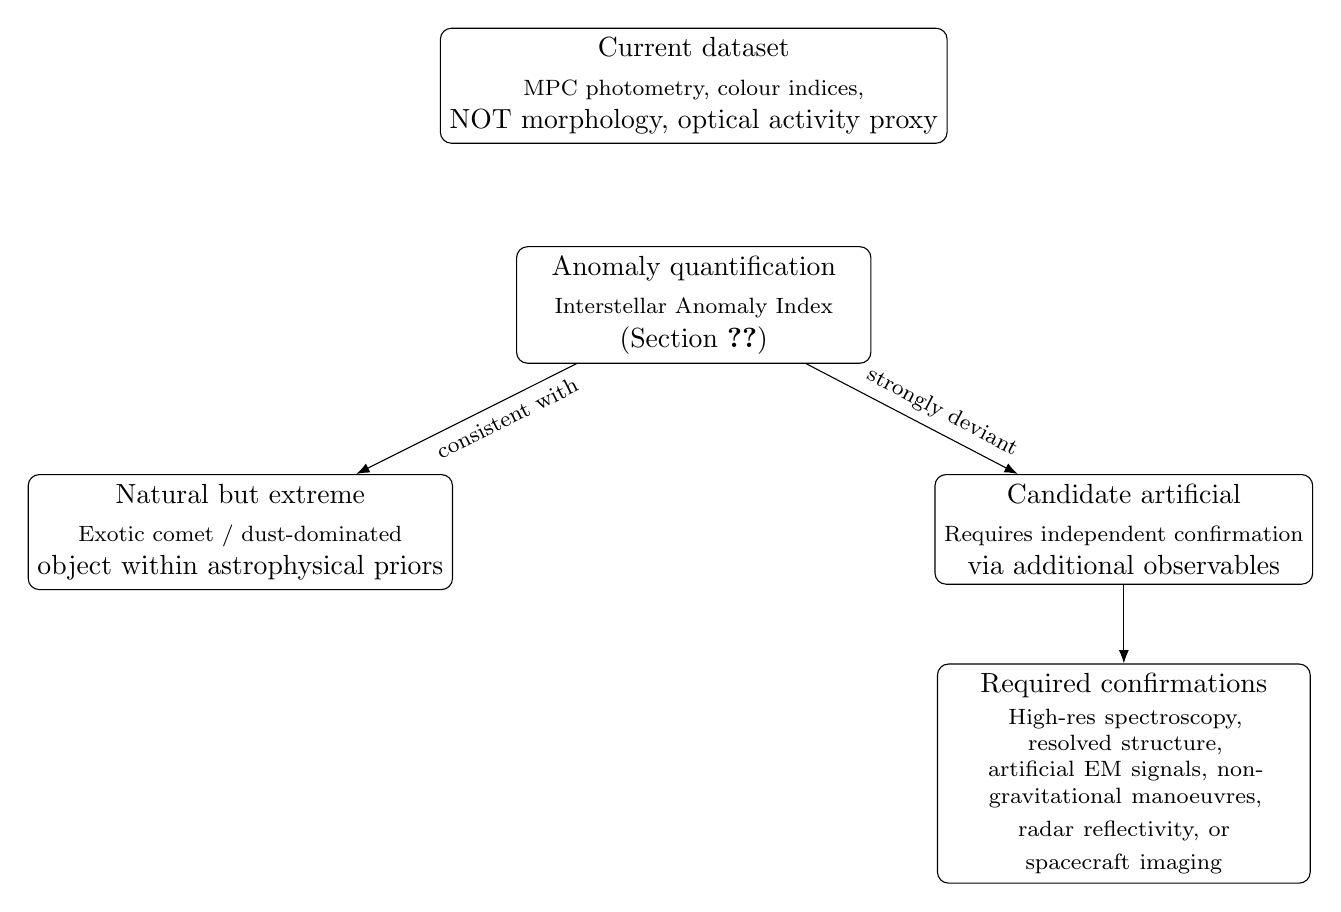
\begin{tikzpicture}[
        node distance=1.3cm and 2.0cm,
        box/.style={rectangle, draw, rounded corners, align=center, minimum width=4.5cm, minimum height=1cm},
        every edge/.style={draw, -Latex}  % Added 'draw' to make arrows visible
    ]

    \node[box] (data) {Current dataset\\[2pt]
        \footnotesize MPC photometry, colour indices,\\
        NOT morphology, optical activity proxy};

    \node[box, below=of data] (anomaly) {Anomaly quantification\\[2pt]
        \footnotesize Interstellar Anomaly Index\\
        (Section~\ref{sec:anomaly_index})};

    \node[box, below left=1.4cm and 0.8cm of anomaly] (natural) {Natural but extreme\\[2pt]
        \footnotesize Exotic comet / dust-dominated\\
        object within astrophysical priors};

    \node[box, below right=1.4cm and 0.8cm of anomaly] (candidate) {Candidate artificial\\[2pt]
        \footnotesize Requires independent confirmation\\
        via additional observables};

    \node[box, below=1.0cm of candidate, text width=4.5cm] (evidence) {Required confirmations\\[2pt]
        \footnotesize High-res spectroscopy, resolved structure,\\
        artificial EM signals, non-gravitational manoeuvres,\\
        radar reflectivity, or spacecraft imaging};

    \draw (anomaly) edge node[midway, below, sloped, pos=0.35]{\footnotesize consistent with} (natural);
    \draw (anomaly) edge node[midway, above, sloped, pos=0.6]{\footnotesize strongly deviant} (candidate);
    \draw (candidate) edge (evidence);

    \end{tikzpicture}
    \caption{Schematic decision pathways from the present photometric analysis to a potential artificial-origin claim. The current work constrains 3I/ATLAS to be highly anomalous with respect to typical cometary behaviour (Section~\ref{sec:anomaly_index}), but cannot by itself cross the threshold to artificial origin. That transition would require independent evidence from spectroscopy, high-resolution imaging, electromagnetic monitoring, non-gravitational manoeuvres without mass loss, radar reflectivity, or in-situ spacecraft observations.}
    \label{fig:artificiality_flow}
\end{figure}

The analysis presented in this work relies primarily on publicly available photometric and multi-filter colour indices from the Minor Planet Center (MPC), combined with post-perihelion morphological imaging and a derived optical activity proxy. These datasets are well suited to the identification of photometric, chromatic, and dynamical anomalies. Indeed, the results of Sections~3–4 demonstrate that 3I/ATLAS exhibits several behaviours inconsistent with typical Solar System comets: an anomalously steep pre-perihelion brightening ($\Delta m \approx 4.2$\,mag), a strong reddening event ($\Delta(g-o)\approx +0.7$\,mag), delayed non-gravitational acceleration, and post-perihelion point-like morphology despite the implied mass loss.\footnote{See Sections~3.3--3.7 for a detailed discussion of these trends.}

However, photometric and colour data alone are not sufficient to determine the \emph{nature} of an 
interstellar object. In particular, they cannot distinguish between a naturally unusual body (e.g., volatile-poor, dust-dominated, compositionally exotic) and one with an artificial or technological origin. This limitation is inherent to the type of data analysed: photometry provides integrated flux information and temporal evolution, but no direct constraints on material composition, structural geometry, surface reflectance properties at high resolution, or electromagnetic signatures. For this reason, the anomaly indices introduced in Section~\ref{sec:anomaly_index} should be interpreted as quantitative measures of \emph{deviation from typical cometary behaviour}, not as direct indicators of artificiality.

\subsubsection{Decision Pathways to Artificial Origin}

It is useful to distinguish conceptually between (i) the detection of anomalous behaviour in photometry and morphology, and (ii) the much stronger requirement of establishing artificial origin. Figure~\ref{fig:artificiality_flow} summarises the logical relationship between the present work and the additional observational channels that would be required to move beyond an anomaly 
classification.

\subsubsection{Data Required for Determination of Artificial Origin}

To assess whether an interstellar object is artificial, one requires evidence that cannot be produced by known natural processes. Several independent observational channels would provide such discrimination, none of which are available in the present dataset:

\begin{enumerate}
    \item \textbf{High-resolution spectroscopy}.  
    Wavelength-resolved spectroscopy is essential for detecting materials with no known natural formation pathway (e.g., engineered alloys, ultra-pure metals, polymers, layered composites, or doped semiconductors). In the case of 3I/ATLAS, published spectral line 
    data remain limited to summary reports (e.g., Ni\,I/Fe\,I abundance anomalies), with no publicly released line lists or calibrated flux tables. Without these data, it is impossible to evaluate whether the observed material is consistent with natural astrophysical environments 
    or indicative of fabrication.

    \item \textbf{Resolved structural imaging}.  
    Determining artificial origin requires imaging capable of revealing geometric features incompatible with natural fragmentation or outgassing. These include: planar surfaces, right-angle edges, periodic structures, symmetric frameworks, or specular (mirror-like) 
    reflections. Current imaging of 3I/ATLAS (e.g., NOT observations) shows a point-like morphology, but the resolution is insufficient to identify or rule out engineered structure.

    \item \textbf{Electromagnetic emissions}.  
    Artificial sources may emit narrowband or modulated radio, microwave, or optical signals that cannot be produced by thermal or chemical processes. SETI criteria classify narrowband ($<1$\,Hz) carriers or structured time-domain modulation as unambiguously artificial. 
    No such observations are presently available for 3I/ATLAS.

    \item \textbf{Non-gravitational manoeuvring without mass loss}.  
    If an object exhibits sustained or repeated changes in trajectory that cannot be explained by outgassing, solar radiation pressure, or other physical mechanisms, artificial propulsion or control becomes the only plausible explanation. While 3I/ATLAS does exhibit non-gravitational acceleration, the absence of simultaneous high-resolution spectral or gas-production data prevents assessment of whether this acceleration is physically consistent with natural mass loss.

    \item \textbf{Radar reflectivity and albedo at microwave wavelengths}.  
    Radar observations can identify metallic or composite materials through anomalously high radar cross-sections or specular reflectance characteristics. No radar detections of 3I/ATLAS have been reported.
\end{enumerate}

\subsubsection{Interpretation of Current Results}

The photometric–chromatic anomalies identified here place 3I/ATLAS among the most unusual interstellar objects observed to date. The combination of steep brightening, transient reddening, delayed dynamical acceleration, and
post-perihelion stellar morphology suggests that the object 
underwent a brief and atypical activation episode whose physical driver is not yet understood. Nevertheless, in the absence of spectroscopy, high-resolution imaging, or electromagnetic monitoring, the present dataset does not permit a conclusion regarding artificial origin.

What can be established is that 3I/ATLAS falls outside the behavioural envelope of typical comets on multiple independent axes. This motivates the development of the anomaly index introduced in Section~\ref{sec:anomaly_index} and underscores the need for comprehensive, multi-instrument 
follow-up of future interstellar visitors. The individual component values and their contribution to the overall index are shown in Figure~\ref{fig:anomaly_components}. Confirmation of artificial origin requires observational signatures that are beyond the scope of photometric analysis and must be obtained through coordinated spectroscopic, imaging, radar, and electromagnetic campaigns.

\begin{figure}[htbp]
    \centering
    \includegraphics[width=0.6\textwidth]{atlas_anomaly_components.png}
    \caption{Normalised anomaly components ($A_{\mathrm{p}}, A_{\mathrm{c}}, A_{\mathrm{a}}, A_{\mathrm{m}}$) 
    for 3I/ATLAS, as defined in Section~\ref{sec:anomaly_index}. All four axes lie near the maximally anomalous regime, yielding an overall Interstellar Anomaly Index of 
    $\mathrm{IAI}_{\mathrm{ATLAS}} \approx 0.95$.}
    \label{fig:anomaly_components}
\end{figure}

The individual component values used in this work, and their contribution to the overall IAI, are summarised in Table~\ref{tab:iai_components}.

\begin{table}[htbp]
\centering
\caption{Illustrative anomaly components and Interstellar Anomaly Index (IAI) values for representative Solar System comet classes and interstellar objects. Component values for 3I/ATLAS are computed directly from the metrics defined in Section~\ref{sec:anomaly_index}. Values for the other objects and classes are approximate, based on published photometric, chromatic, dynamical, and morphological behaviour, and are intended as fiducial placements within the $(e,\mathrm{IAI})$ plane rather than results of a full re-analysis.}
\label{tab:iai_components}
\begin{tabular}{lccccc}
\toprule
\textbf{Object / Class} & $A_{\mathrm{p}}$ & $A_{\mathrm{c}}$ & $A_{\mathrm{a}}$ & $A_{\mathrm{m}}$ & $\mathrm{IAI}$ \\
\midrule
Typical JFC      & 0.10 & 0.00 & 0.00 & 0.00 & 0.03 \\
Typical LPC      & 0.20 & 0.10 & 0.00 & 0.00 & 0.08 \\
1I/\textit{'Oumuamua} & 0.00 & 0.00 & 1.00 & 0.80 & 0.45 \\
2I/Borisov       & 0.20 & 0.10 & 0.25 & 0.10 & 0.16 \\
\textbf{3I/ATLAS} & \textbf{0.90} & \textbf{1.00} & \textbf{1.00} & \textbf{0.90} & \textbf{0.95} \\
\bottomrule
\end{tabular}
\end{table}

% =======================================================
\section{Data Integrity and Reproducibility}
% =======================================================
All scripts, CSV outputs, and figures were archived in a public GitHub repository with versioned manifests:
\begin{itemize}
\item \texttt{watch\_mpc\_colors\_plot\_v\_8\_4.py} — colour/solar comparison pipeline
\item \texttt{atlas\_optical\_acceleration\_v2.py} — acceleration extraction and smoothing
\item \texttt{atlas\_optical\_color\_correlation\_v1.py} — composite optical–chromatic analysis
\item \texttt{update\_I3\_data.sh} — automatic MPC update + OpenTimestamps + GPG sealing
\end{itemize}

Each run is recorded in \texttt{RUN\_LOG.md}, listing SHA256 hashes, proof manifests, and timestamps on multiple Bitcoin calendars.

% =======================================================
\section{Conclusion}
% =======================================================
We have presented a detailed photometric, chromatic, and morphological analysis of the interstellar object 3I/ATLAS based on publicly available MPC data, colour indices, and post-perihelion imaging. The results reveal several independent anomalies that are difficult to reconcile with the behavioural envelope of typical Solar System comets. These include an unusually steep pre-perihelion brightening ($\Delta m \approx 4.2$\,mag), a strong transient reddening in $g-o$ colour ($\Delta \approx 0.7$\,mag), a delayed onset of non-gravitational acceleration, and a compact, stellar post-perihelion morphology inconsistent with the level of pre-perihelion activity.

A noteworthy feature of this evolution is the $\sim$4-week offset between the photometric activity peak and the formal detection of non-gravitational acceleration. This demonstrates that optical diagnostics—particularly the optical activity proxy developed here—can provide advance warning of impending dynamical changes in interstellar objects. Combined with the pre-perihelion reddening and the post-perihelion deceleration and fading, the data are consistent with a brief, dust-driven activation episode, possibly reflecting transient surface reconfiguration under solar irradiation.

In Section~\ref{sec:jupiter_dv}, we examined whether the observed optical–acceleration anomaly could generate a trajectory perturbation of the magnitude associated with the proposed near–Hill-radius Jupiter encounter. By scaling the optical acceleration proxy to two physically motivated regimes (a minimal $\Delta v_{\mathrm{tot}} = 8~\mathrm{m\,s^{-1}}$ and a photometric $\Delta v_{\mathrm{tot}} = 25~\mathrm{m\,s^{-1}}$), we found that short-lived activity bursts on 2025-09-10 and 2025-10-02 dominate the impulse budget and are dynamically capable of producing transverse displacements in the range $(0.05$–$0.31)\times10^{6}$~km, depending on jet angle. These results do not discriminate between natural and non-natural interpretations, but they show that the required dynamical impulse is entirely compatible with the timing and structure of the photometric anomaly.

To quantitatively synthesise the broader set of deviations, we introduced the \emph{Interstellar Anomaly Index} (IAI), a dimensionless measure of multi-axial anomaly strength defined in Section~\ref{sec:anomaly_index}. With $\mathrm{IAI}_{\mathrm{ATLAS}} \approx 0.95$, 3I/ATLAS lies near the maximally anomalous end of the scale, combining very high eccentricity ($e \approx 6.14$) with strongly atypical photometric, chromatic, dynamical, and morphological signatures. In the broader $(e,\mathrm{IAI})$ parameter space, ATLAS occupies an extreme region (Figure~\ref{fig:iai_vs_e}), markedly separated from Jupiter-family comets, long-period comets, and even the first two interstellar objects, 1I/'Oumuamua and 2I/Borisov (Table~\ref{tab:iai_summary}).

These findings do not imply an artificial origin. As emphasised in Section~\ref{sec:limitations_artificiality}, photometry and broadband colour data alone are fundamentally insufficient for determining the physical nature of an interstellar object. Confirmation of technological origin would require independent evidence, such as wavelength-resolved spectroscopy revealing engineered materials, resolved structural imaging, modulated electromagnetic emissions, non-gravitational manoeuvres without mass loss, radar reflectivity indicative of metallic surfaces, or in-situ spacecraft observations.

What can be concluded is that 3I/ATLAS does not fit neatly into existing cometary classifications and exhibits strongly atypical behaviour on multiple independent axes. The anomaly index introduced here provides a reproducible framework for evaluating future interstellar visitors and placing them within a quantitative multi-parameter space. As more interstellar objects enter the Solar System, it will become increasingly possible to determine whether the behaviour of 3I/ATLAS represents an emerging class of interstellar bodies or whether it stands as uniquely unusual among known visitors.

% =======================================================
\begin{thebibliography}{10}
% =======================================================

\bibitem{zenodoV1} Gherbi, Salah-Eddin (2025). \textit{3I/ATLAS (C/2019 Y4) - Photometric Anomaly 2025 - Raw MPC Photometry Analysis} (Version 1.0) [Data set]. Zenodo. \url{https://doi.org/10.5281/zenodo.17477597}

\bibitem{zenodoV2} Gherbi, Salah-Eddin (2025). \textit{3I/ATLAS (C/2019 Y4) - Photometric Anomaly 2025 - Horizons Comparison Extension} (Version 2.0) [Data set]. Zenodo. \url{https://doi.org/10.5281/zenodo.17483027}

\bibitem{zenodoV21} Gherbi, Salah-Eddin (2025). \textit{3I/ATLAS (C/2019 Y4) - Photometric Anomaly 2025 - ZTF Verification} (Version 2.1) [Data set]. Zenodo. \url{https://doi.org/10.5281/zenodo.17487610}

\bibitem{zenodoV22} Gherbi, Salah-Eddin (2025). \textit{3I/ATLAS Photometric–Chromatic Anomaly (2025): Timestamped Dataset and Optical Acceleration Analysis} (Version~2.2) [Data set]. Zenodo. \url{https://doi.org/10.5281/zenodo.17503806}

\bibitem{zenodoV23} Gherbi, Salah-Eddin (2025). \textit{3I/ATLAS Photometric–Chromatic Anomaly (2025): Spectral Transition and Post-Perihelion Evolution} (Version~2.3) [Data set]. Zenodo. \url{https://doi.org/10.5281/zenodo.17538229}

\bibitem{zenodoV24} Gherbi, Salah-Eddin (2025). \textit{3I/ATLAS Photometric–Chromatic Anomaly (2025): Extended MPC Photometry and Post-Perihelion Deceleration} (Version~2.4) [Data set]. Zenodo. \url{https://doi.org/10.5281/zenodo.17609914}

\bibitem{zenodoV25} Gherbi, Salah-Eddin (2025). \textit{3I/ATLAS Photometric–Chromatic Anomaly (2025): Interstellar Anomaly Index and Extended Post-Perihelion Evolution} (Version~2.5) [Data set]. Zenodo. \url{https://doi.org/10.5281/zenodo.17692904}

\bibitem{naves2025} Naves, R. (2025). \textit{No Clear Cometary Tail in Post-Perihelion Images of 3I/ATLAS}. R. Naves Observatory, Spain. Retrieved from: \url{https://avi-loeb.medium.com/no-clear-cometary-tail-in-post-perihelion-images-of-3i-atlas-e3904b352a7a}

\bibitem{loeb2025atlas} Loeb, A. (2025). \textit{Post Perihelion Data on 3I/ATLAS}. Medium. \url{https://avi-loeb.medium.com/post-perihelion-data-on-3i-atlas-3d1e72be2bb4}

\bibitem{atel17490} Jewitt, D., \& Luu, J. (2025). \textit{NOT imaging of interstellar object 3I/ATLAS (C/2025 N1)}. Astronomer's Telegram, 17490. Retrieved from: \url{https://www.astronomerstelegram.org/?read=17490}

\end{thebibliography}

% =======================================================
\section*{Acknowledgements}
The author thanks the Minor Planet Center for public data access, JPL for orbital parameters, and the OpenTimestamps community for cryptographic proof-of-existence infrastructure.

% =======================================================
\section*{Data Availability and Citation}
% =======================================================

All photometric, analytical, and verification materials associated with this study are openly archived on Zenodo:

\begin{quote}
\textbf{Gherbi, Salah-Eddin} (2025). \emph{3I/ATLAS Photometric--Chromatic Anomaly Analysis, Interstellar Anomaly Index, $\Delta v$--Based Dynamical Assessment, and Extended Post--Perihelion Evolution} (Version~2.5).  
Zenodo. \url{https://doi.org/10.5281/zenodo.17692904}
\end{quote}

This repository contains the complete \textbf{v2.5 proof bundle}, including all Python analysis scripts, processed datasets, figures, LaTeX source files, and reproducibility artefacts:

\begin{itemize}
  \item \textbf{Python analysis scripts}  
    \begin{itemize}
      \item \texttt{watch\_mpc\_colors\_plot\_v\_8\_4.py}  
      \item \texttt{atlas\_optical\_acceleration\_v2.py}  
      \item \texttt{atlas\_optical\_color\_correlation\_v1.py} 
      \item \texttt{iai\_vs\_eccentricity.py}  
      \item \texttt{atlas\_anomaly\_index.py}
       \item \texttt{atlas\_delta\_v\_from\_optical\_proxy.py}  
      \item \texttt{atlas\_optical\_dv\_dual.py}  
      \item \texttt{plot\_atlas\_optical\_accel\_deltav.py}
    \end{itemize}

  \item \textbf{Automation and integrity scripts}  
    \begin{itemize}
      \item \texttt{update\_I3\_data.sh}  
      \item \texttt{append\_run\_log\_v3.sh}  
    \end{itemize}

  \item \textbf{Processed datasets (CSV)}  
    \begin{itemize}
      \item \texttt{I3\_Color\_Alerts\_*.csv}  
      \item \texttt{I3\_Optical\_Acceleration\_Data.csv}  
    \end{itemize}

  \item \textbf{Figures generated in v2.5}  
    \begin{itemize}
      \item \texttt{I3\_Optical\_Acceleration\_Trend\_v2.png}  
      \item \texttt{I3\_Optical\_Color\_Correlation.png}  
      \item \texttt{I3\_Optical\_Color\_Correlation\_postperi.png}  
      \item \texttt{atlas\_anomaly\_components.png}  
      \item \texttt{iai\_vs\_eccentricity.png}
      \item \texttt{I3\_Optical\_Acceleration\_DeltaV\_Figure.png}
      \item \texttt{I3\_Optical\_Acceleration\_DeltaV\_8\_vs\_25.png}
      \item \texttt{I3\_Optical\_Acceleration\_DeltaV\_Overlay.png}
    \end{itemize}

  \item \textbf{Source and documentation}  
    \begin{itemize}
      \item \texttt{3I\_ATLAS\_Anomaly\_2025.tex}  
      \item \texttt{I3\_ATLAS\_v2\_5\_Analysis.pdf}  
      \item \texttt{README\_PROOF\_v2\_5.md}  
    \end{itemize}

  \item \textbf{Cryptographic verification artefacts}  
    \begin{itemize}
      \item \texttt{RUN\_LOG.md}  
      \item All associated \texttt{.asc} GPG signatures  
      \item All associated \texttt{.ots} OpenTimestamps proofs  
    \end{itemize}
\end{itemize}

All files are timestamped on the Bitcoin blockchain using \textbf{OpenTimestamps} and digitally signed via \textbf{GPG}, providing a verifiable proof-of-existence and authorship trail for every versioned component of the analysis.

The dataset is released under the \href{https://creativecommons.org/licenses/by-nc/4.0/}{CC~BY–NC~4.0} license.

\end{document}
